\chapter{Supplementary Figures}

\begin{figure}[htb!]
    \centering
    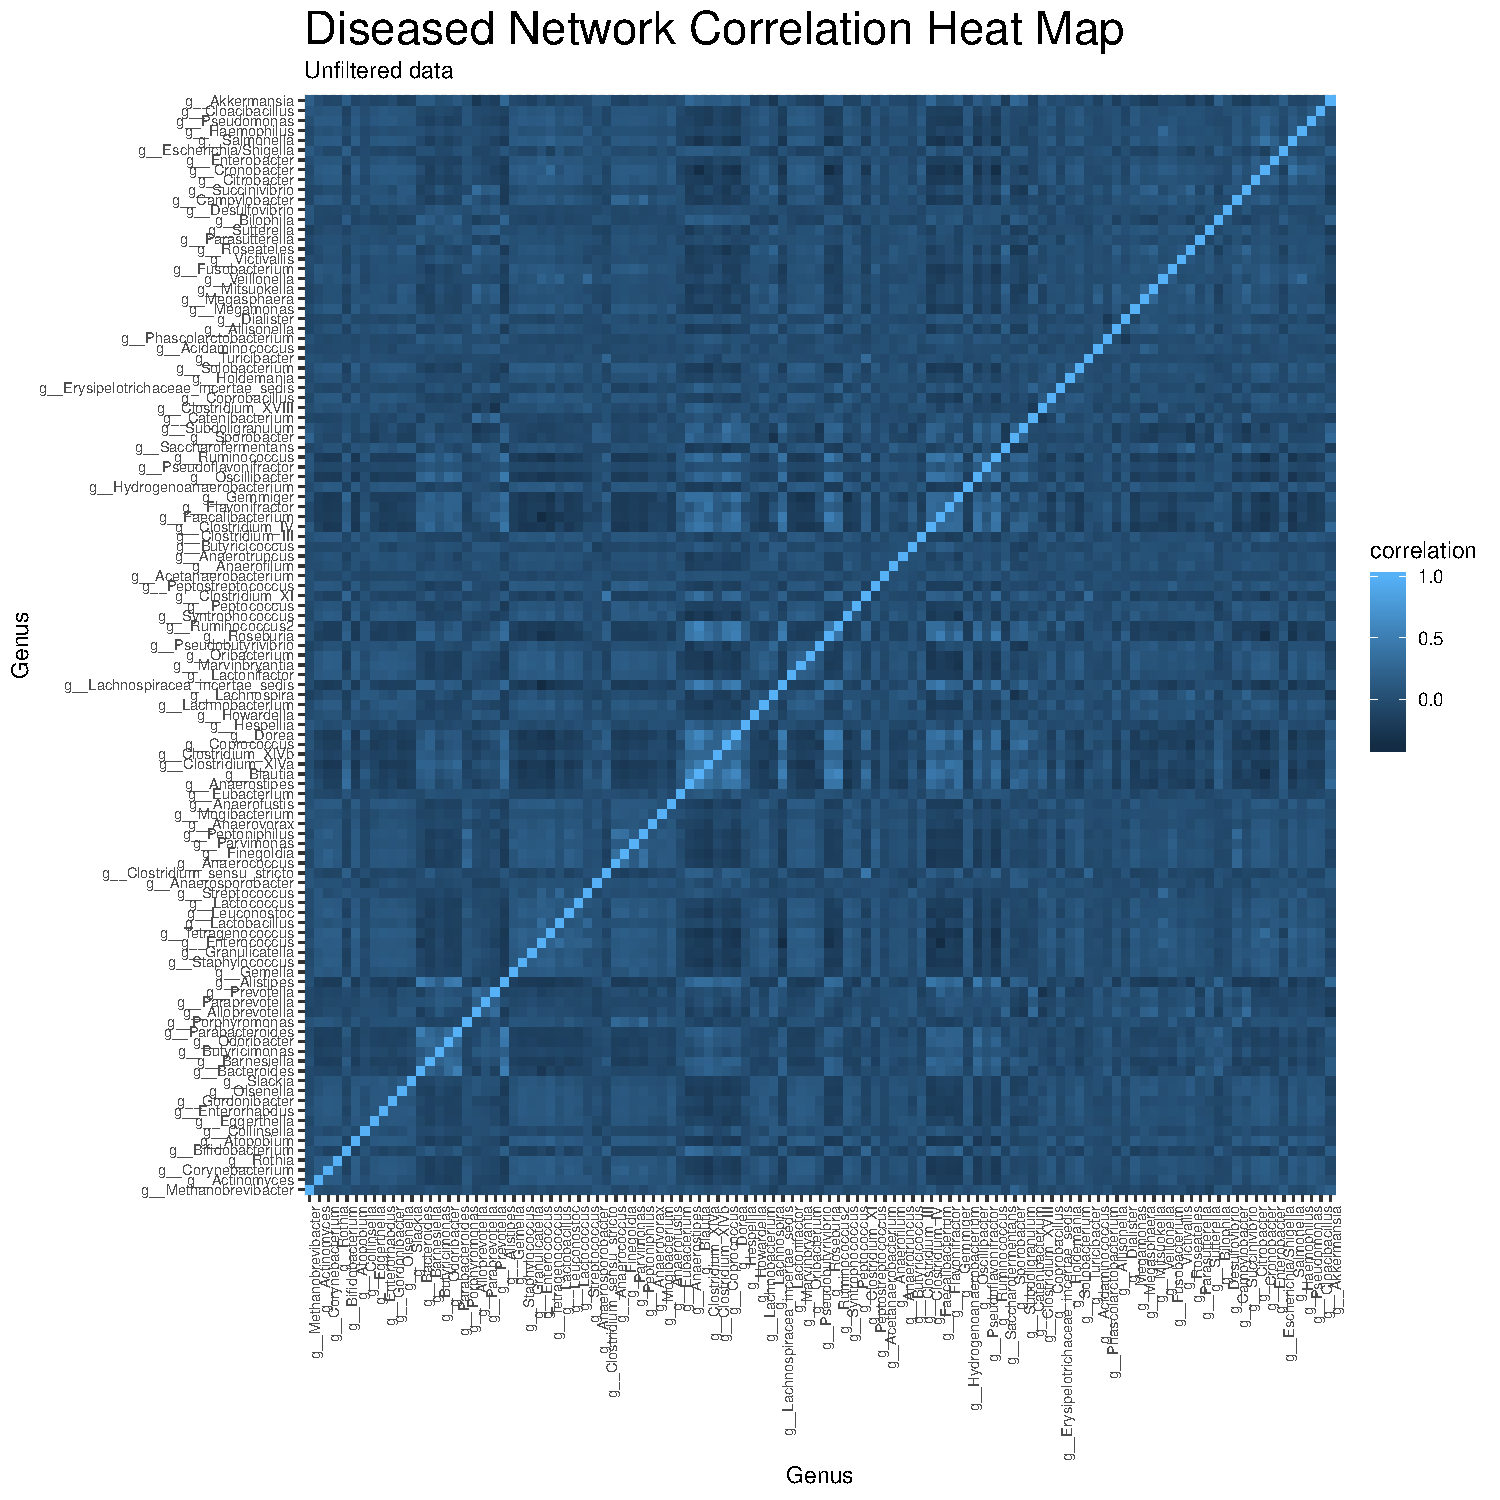
\includegraphics[width=1.0\linewidth]{figure/results/diseased_raw_corr_heatmap.pdf}
    \caption[Heat map of the resulting diseased FastSpar correlation matrix.]{Heat map of the resulting diseased FastSpar correlation matrix. Genera are listed on the respective axes and correlation values are colored based upon their strength. }
    \label{apdx-fig-d-orig-heatmap}
\end{figure}

\begin{figure}[!hbtp]
\centering
\subfloat[Degree distribution for the filtered healthy and diseased networks and the overlapping sub-graphs.]{
    \label{subfig:deg_dist}
    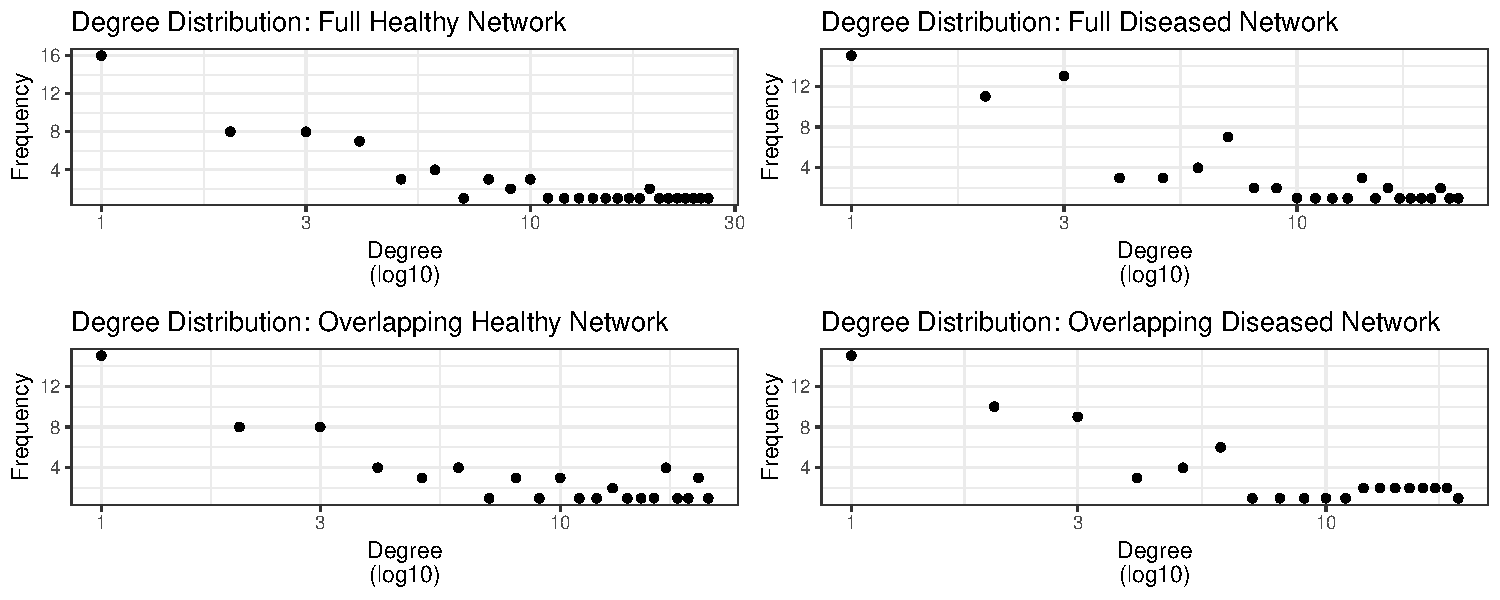
\includegraphics[width=0.94\textwidth]{figure/results/degree_plots.pdf}}
    \hfill
\subfloat[Betweenness centrality distribution for the filtered healthy and diseased networks and the overlapping sub-graphs]{
    \label{subfig:btween_dist}
    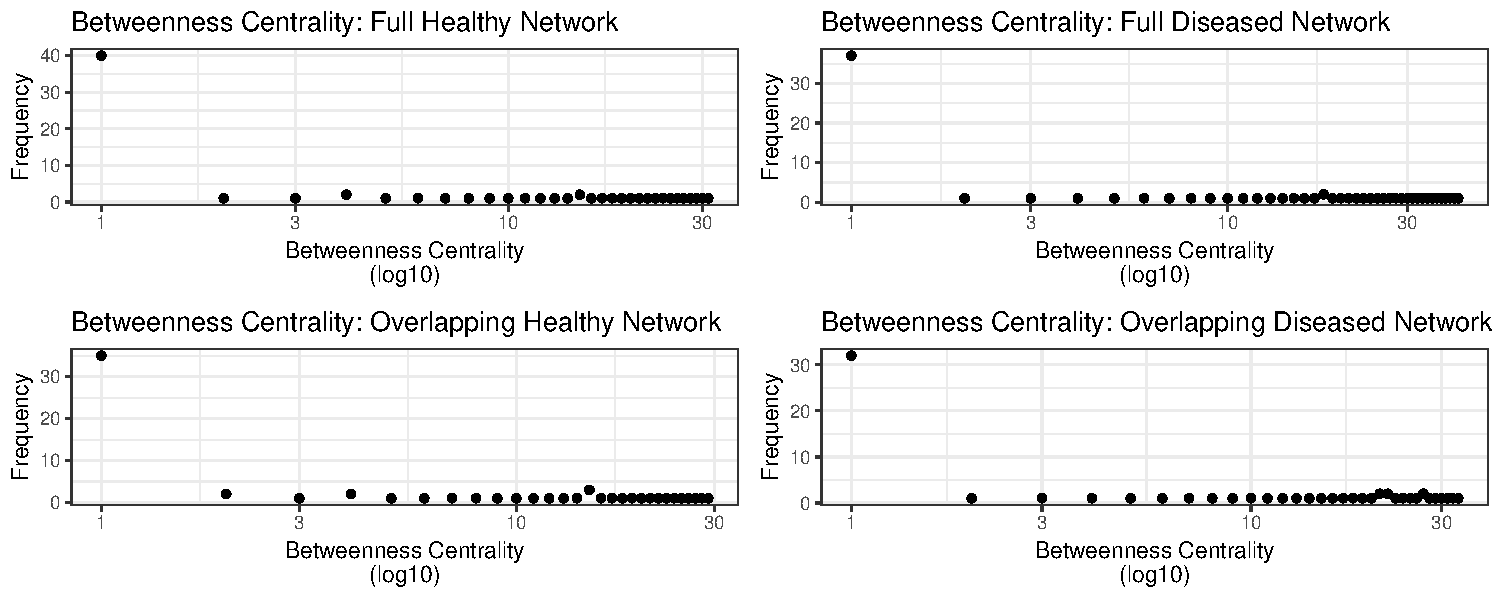
\includegraphics[width=0.94\textwidth]{figure/results/btween_plots.pdf}}
    \hfill
\subfloat[Coreness centrality distribution for the filtered healthy and diseased networks and the overlapping sub-graphs]{
    \label{subfig:core_dist}
    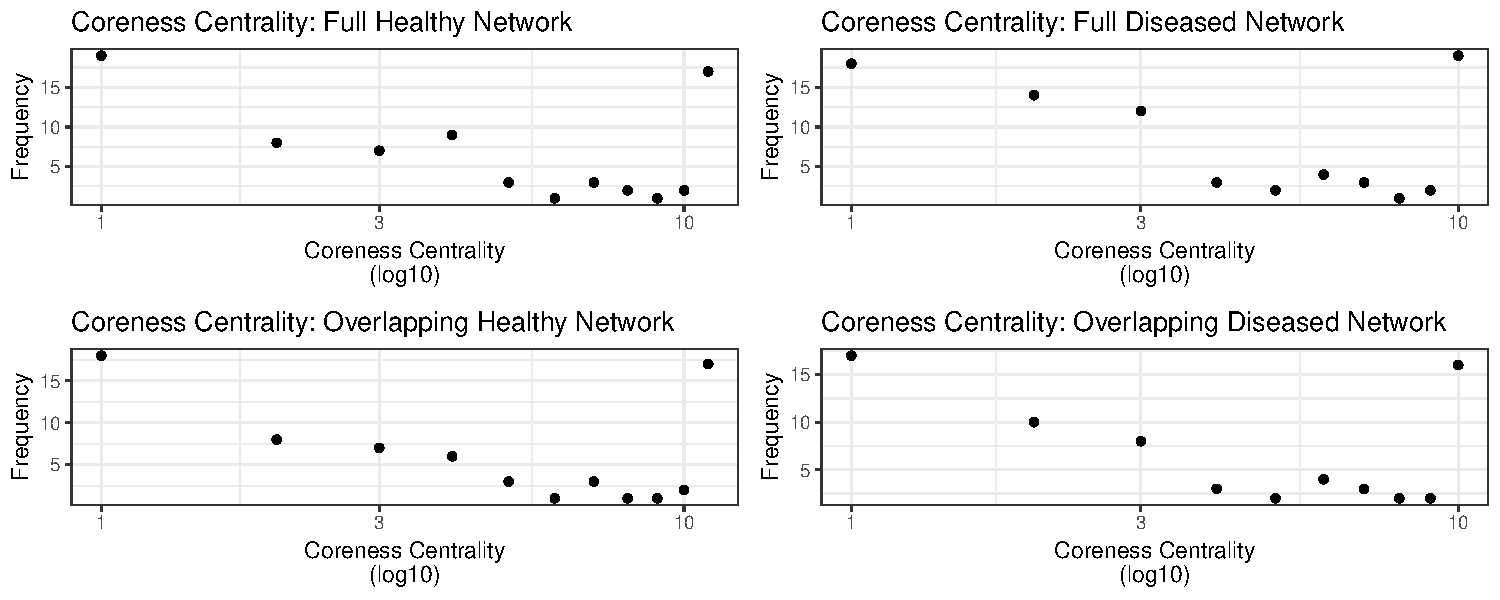
\includegraphics[width=0.94\textwidth]{figure/results/core_plots.pdf}}
\caption[Degree, betweenness centrality, and coreness centrality distributions for the filtered healthy and diseased networks.]{Distributions mentioned in Section \ref{results-netstat} for the filtered healthy and diseased networks. \textbf{(a)} contains the degree distributions, \textbf{(b)} contains the betweenness centrality distributions, and \textbf{(c)} contains the coreness centrality distributions.}
\label{fig:dist_plots}
\end{figure}

\begin{table}[!hbtp]
\centering
\begin{tabular}{rll}
  \toprule
 & Degree FHN & Degree FDN \\ 
  \midrule
Rank 1 & 38,  g\_Clostridium\_IV & 40,  g\_Clostridium\_IV \\ 
  Rank 2 & 33,  g\_Clostridium\_XlVa & 30,  g\_Coprococcus \\ 
  Rank 3 & 32,  g\_Blautia & 29,  g\_Clostridium\_XlVa \\ 
  Rank 4 & 31,  g\_Coprococcus & 29,  g\_Ruminococcus \\ 
  Rank 5 & 29,  g\_Gemmiger & 28,  g\_Blautia \\ 
  \midrule
%   \bottomrule
% \end{tabular}
% \label{tab:fhn_fdn_centrality}
% \end{table}

% \begin{table}[ht]
% \centering
% \begin{tabular}{rll}
%   \hline
 & Degree OHN & Degree ODN \\ 
  \midrule
Rank 1 & 35,  g\_Clostridium\_IV & 35,  g\_Clostridium\_IV \\ 
  Rank 2 & 29,  g\_Blautia & 27,  g\_Coprococcus \\ 
  Rank 3 & 29,  g\_Clostridium\_XlVa & 27,  g\_Ruminococcus \\ 
  Rank 4 & 29,  g\_Coprococcus & 26,  g\_Blautia \\ 
  Rank 5 & 27,  g\_Ruminococcus & 26,  g\_Clostridium\_XlVa \\ 
%   \bottomrule
% \end{tabular}
% \end{table}
\bottomrule \toprule
% \begin{table}[ht]
% \centering
% \begin{tabular}{rll}
%   \toprule
 & Betweenness Centrality FHN & Betweenness Centrality FDN \\ 
  \midrule
Rank 1 & 504,  g\_Clostridium\_IV & 626,  g\_Clostridium\_IV \\ 
  Rank 2 & 489,  g\_Blautia & 577,  g\_Coprococcus \\ 
  Rank 3 & 319,  g\_Clostridium\_XlVa & 344,  g\_Clostridium\_XlVa \\ 
  Rank 4 & 308,  g\_Oscillibacter & 324,  g\_Blautia \\ 
  Rank 5 & 254,  g\_Faecalibacterium & 250,  g\_Faecalibacterium \\ 
  \midrule
  
 & Betweenness Centrality OHN & Betweenness Centrality ODN \\ 
  \midrule
Rank 1 & 428,  g\_Blautia & 438,  g\_Clostridium\_IV \\ 
  Rank 2 & 388,  g\_Clostridium\_IV & 297,  g\_Blautia \\ 
  Rank 3 & 294,  g\_Oscillibacter & 222,  g\_Clostridium\_XlVa \\ 
  Rank 4 & 249,  g\_Clostridium\_XlVa & 205,  g\_Faecalibacterium \\ 
  Rank 5 & 221,  g\_Sporobacter & 203,  g\_Coprococcus \\ 
%   \bottomrule
% \end{tabular}
% \end{table}
\bottomrule \toprule
% \begin{table}[ht]
% \centering
% \begin{tabular}{rll}
%   \toprule
 & Coreness Centrality FHN & Coreness Centrality FDN \\ 
  \midrule
Rank 1 & 12,  g\_Alistipes & 11,  g\_Alistipes \\ 
  Rank 2 & 12,  g\_Anaerostipes & 11,  g\_Tetragenococcus \\ 
  Rank 3 & 12,  g\_Blautia & 11,  g\_Anaerostipes \\ 
  Rank 4 & 12,  g\_Clostridium\_XlVa & 11,  g\_Blautia \\ 
  Rank 5 & 12,  g\_Coprococcus & 11,  g\_Clostridium\_XlVa \\ 
   \midrule
   
 & Coreness Centrality OHN & Coreness Centrality ODN \\ 
  \midrule
Rank 1 & 12,  g\_Alistipes & 11,  g\_Alistipes \\ 
  Rank 2 & 12,  g\_Anaerostipes & 11,  g\_Anaerostipes \\ 
  Rank 3 & 12,  g\_Blautia & 11,  g\_Blautia \\ 
  Rank 4 & 12,  g\_Clostridium\_XlVa & 11,  g\_Clostridium\_XlVa \\ 
  Rank 5 & 12,  g\_Coprococcus & 11,  g\_Coprococcus \\ 
   \bottomrule
\end{tabular}
\caption{Table mentioned in Section \ref{results-netstat} listing the five genera that have the highest degree, betweenness centrality, and coreness centrality for the \acrfull{FHN}, \acrfull{FDN}, \acrfull{OHN}, and \acrfull{ODN}.}
\label{tab:node-measures}
\end{table}

\begin{figure}[htb!]
    \centering
    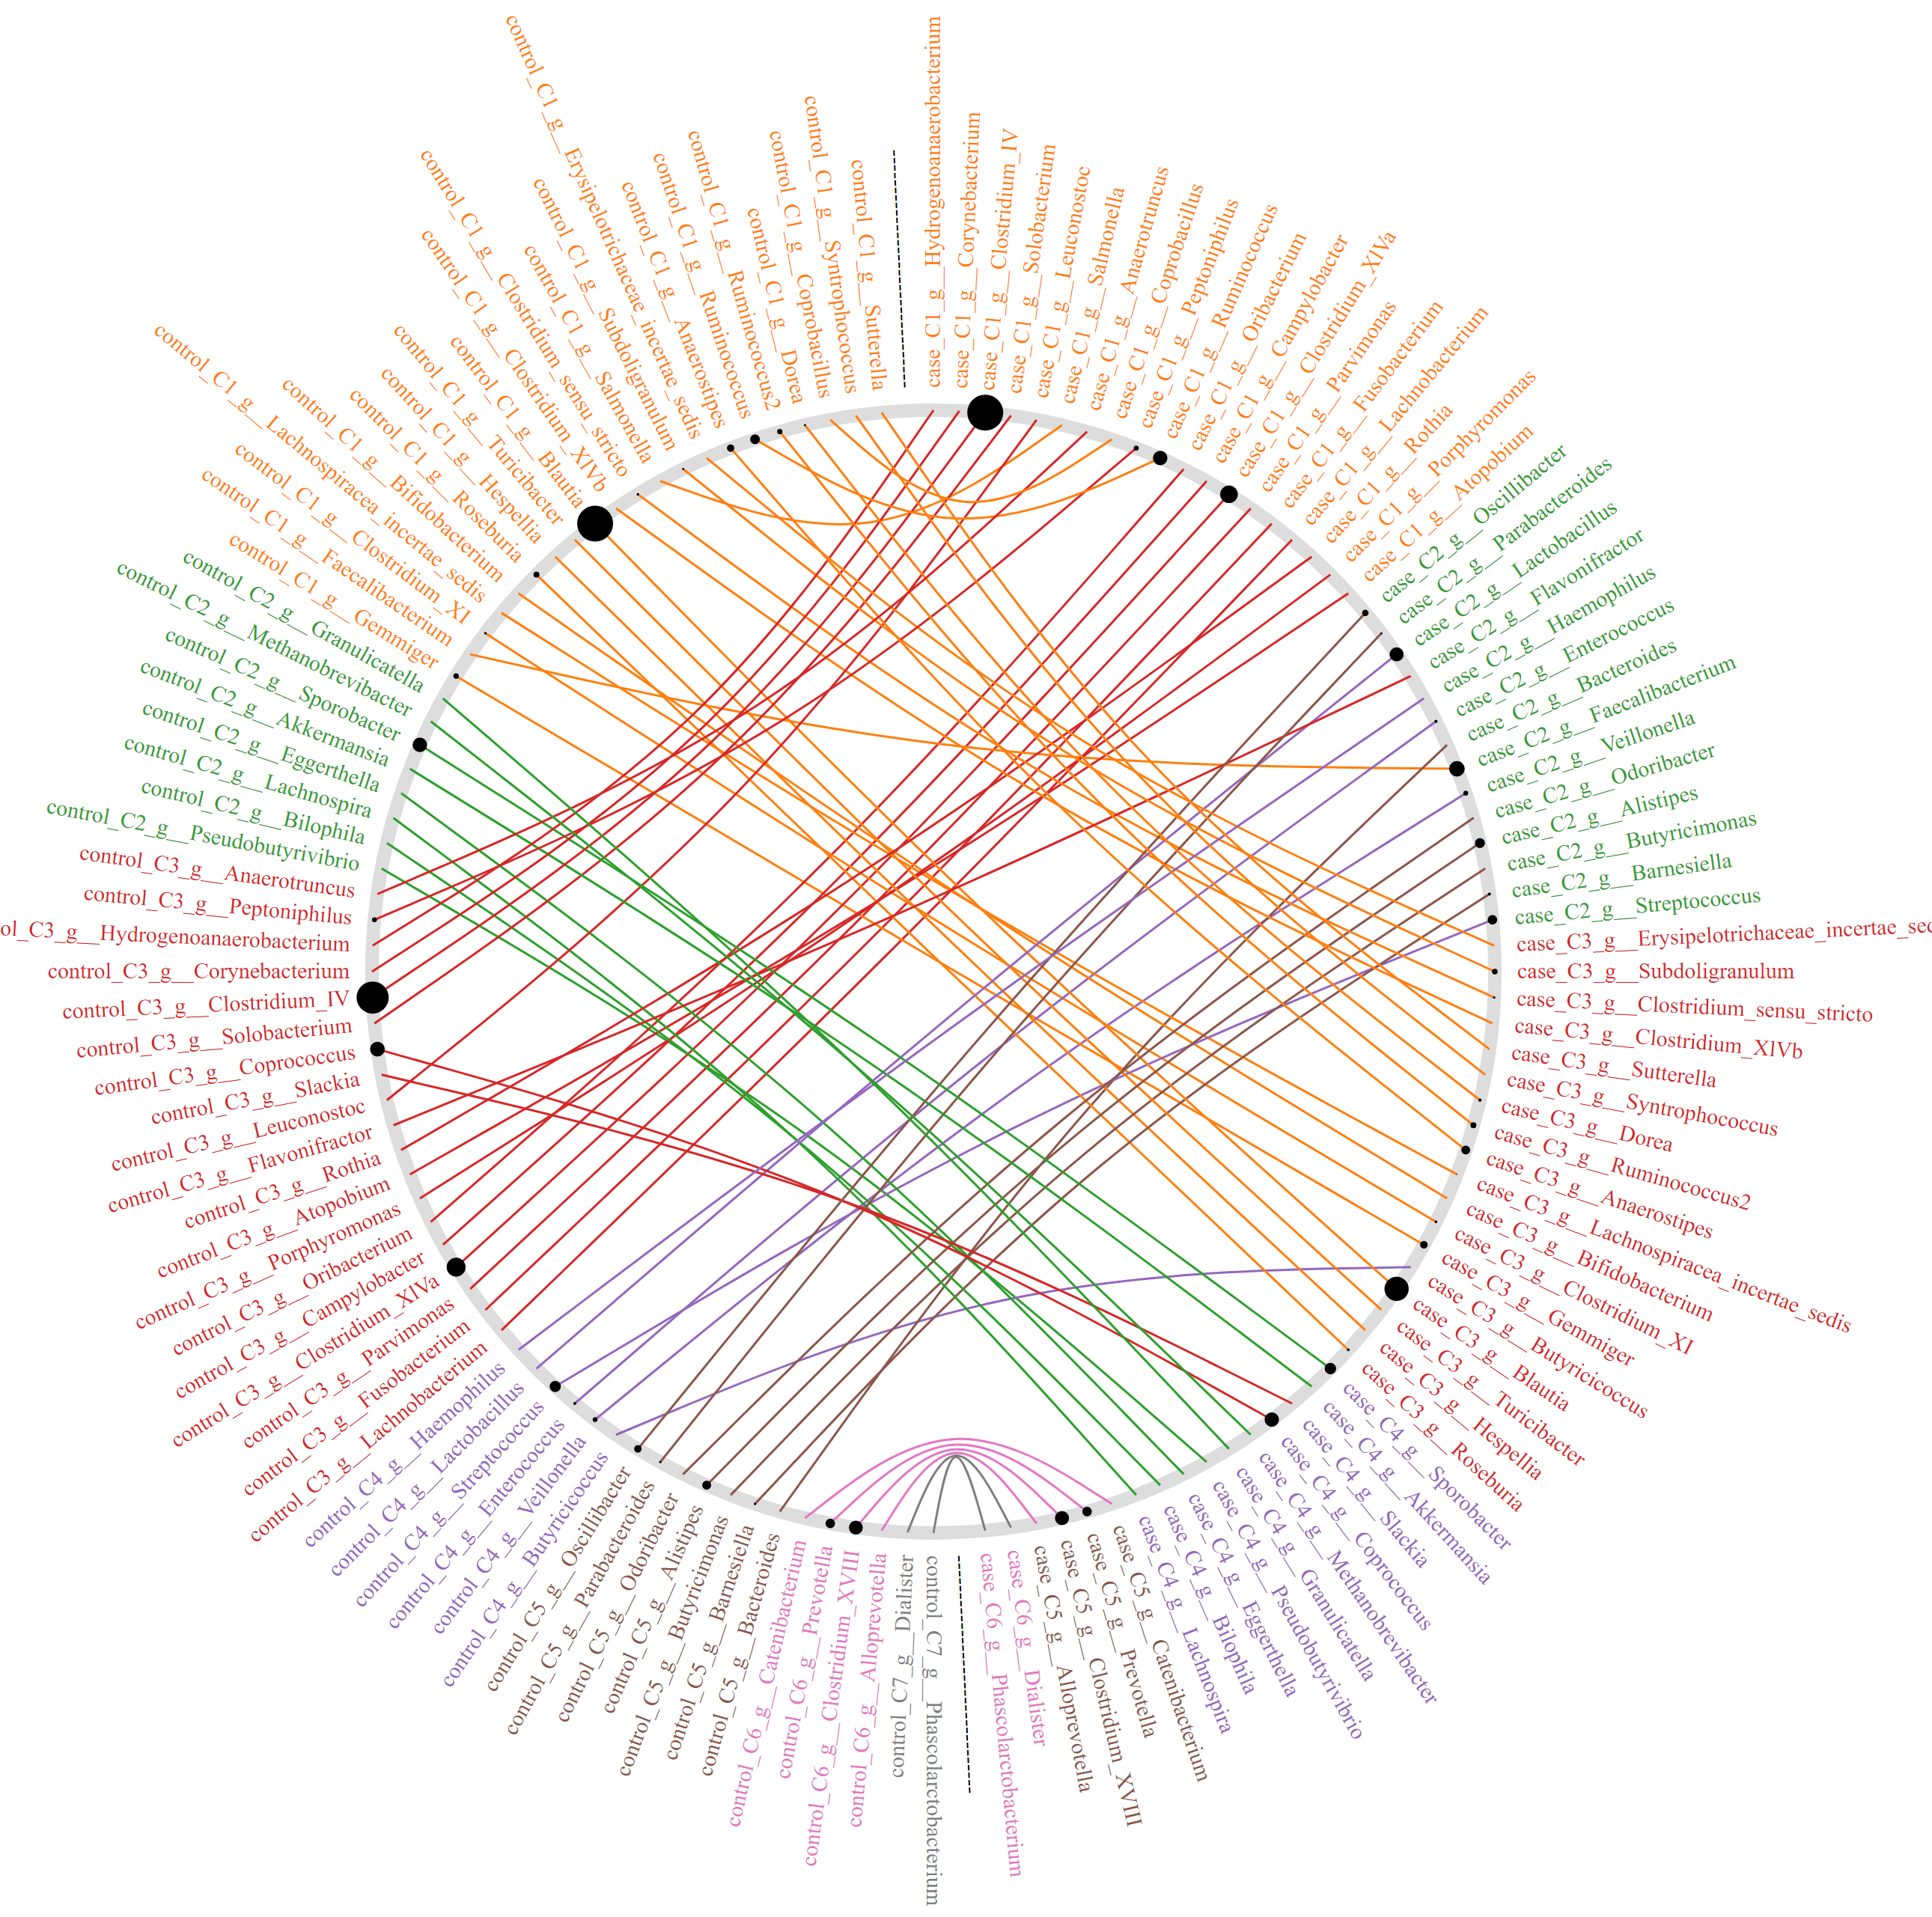
\includegraphics[width=1.0\linewidth]{figure/results/shuffle_net.png}
    \caption[The full NetShift shuffle diagram highlighting re-wiring between communities identified by hierarchical clustering.]{The full NetShift shuffle diagram highlighting re-wiring between communities identified by hierarchical clustering mentioned in Section \ref{res:shift}. All taxa are represented by the control taxa on the left of the diagram and case taxa on the right. Communities are identified by the color of the taxon. The shuffle plot in Figure \ref{fig:res-shuffle} can be useful to interpret this diagram.}
    \label{apdx-nesh-shuffle}
\end{figure}
